\section{Bias-variance Limits: Different Sample Sizes and Covariate Shifts}\label{sec_diff}

The previous section assumes that all tasks have the same sample size and feature vectors.
In this section, we study how different sample sizes and different features impact hard parameter sharing.
%The different covariates case differs from the same covariates case in two aspects.
%First, different tasks may have different sample sizes. In extreme scenarios, one task may have much less labeled data compared to another task.
The setting where features differ across tasks is often called ``covariate shift''.

Unlike the previous section, we no longer have an optimal solution to $f(A, B)$.
This is because $f(A, B)$ is in general non-convex.
Instead, our result implies tight generalization bounds for any \emph{local minimizer} of $f(A, B)$.
We focus on the two-task case to better understand the impact of having different sample sizes and different covariates.
Suppose that $X^{(1)} = Z^{(1)}(\Sigma^{(1)})^{1/2} \in \real^{n_1 \times p}$ and $X^{(2)} = Z^{(2)}(\Sigma^{(2)})^{1/2} \in \real^{n_2 \times p}$, where the entries of $Z^{(1)}$ and $ Z^{(2)}$ are drawn independently from a one dimensional distribution with zero mean, unit variance, and constant $\varphi$-th moment for a fixed $\varphi > 4$. The matrices $\Sigma^{(1)}\in \R^{p\times p}$ and $\Sigma^{(2)}\in \R^{p\times p}$ denote the population covariance matrices of task 1 and task 2, respectively.

\paragraph{Bias-variance equations.}
Our key result characterizes the asymptotic limit of the inverse of the sum of two different sample covariance matrices.
Without loss of generality, we consider task two's prediction loss and the same result applies to task one.
By Proposition 1 of \citet{WZR20}, we consider the case of $r = 1 < t = 2$, since when $r > 1$, the optimal solution of $f(A, B)$ is equivalent to single-task learning.
When $r = 1$, $B$ is a vector and $A_1, A_2$ are both scalars.
To motivate our study, we consider a special case where $A_1=A_2=1$. 
%Hence we can write down a closed form equation for any local minimizer of $f(A, B)$.
By solving $B$ in equation \eqref{eq_mtl}, we obtain the hard parameter sharing estimator $\hat{\beta}_2^{\MTL} = B A_2 = B$ as follows:
\begin{align}
	\hat{\beta}_2^{\MTL} &= {\hat{\Sigma}}^{-1} ({X^{(1)}}^{\top} Y^{(1)} + {X^{(2)}}^{\top} Y^{(2)}), \ \ \text{ where } \nonumber \\
	\hat{\Sigma} &= {X^{(1)}}^{\top} X^{(1)} + {X^{(2)}}^{\top} X^{(2)}. \label{def hatsig}
\end{align}
The matrix $\hat{\Sigma}$ adds up both tasks' sample covariance matrices, and the expectation of $\hat{\Sigma}$ is equal to a mixture of their population covariance matrices, with mixing proportions determined by their sample sizes.

To derive the bias and variance equation, we consider the expected loss conditional on the covariates as follows (the empirical loss is close to its expectation similar to Claim \ref{claim_pred_err}):
\begin{align}
	& \exarg{\cE}{L(\hat{\beta}_2^{\MTL}) \mid X^{(1)}, X^{(2)}}  \nonumber \\
	=& \bignorm{{\Sigma^{(2)}}^{1/2} \hat{\Sigma}^{-1} {X^{(1)}}^{\top} X^{(1)} (\beta^{(1)} - \beta^{(2)})}^2 \label{eq_bias_2task} \\
	& + \sigma^2 \bigtr{\Sigma^{(2)}\hat{\Sigma}^{-1}}. \label{eq_variance_2task}
\end{align}
Equation \eqref{eq_bias_2task} and \eqref{eq_variance_2task} correspond to the bias and variance of hard parameter sharing for two tasks, respectively.
Our main result in this section characterizes the asymptotic bias-variance limits under the high-dimensional assumption.
Intuitively, the spectrum of $\hat{\Sigma}^{-1}$ (and hence its trace) not only depends on both tasks' sample sizes, but also depends on the ``alignment'' between $\Sigma^{(1)}$ and $\Sigma^{(2)}$.
However, capturing this intuition quantitatively turns out to be technically challenging.
%The main technical challenge of our result deals with the ``covariate shift'' between tasks one and two.
We introduce a key quantity $M \define (\Sigma^{(1)})^{1/2}(\Sigma^{(2)})^{-1/2}$, and as we show below, the trace of $\hat{\Sigma}^{-1}$ has an intricate dependence on the spectrum of $M$.

Let $U\Lambda V^\top$ denote the SVD of $M$ and let $\lambda_1, \lambda_2, \dots, \lambda_p$ denote $M$'s singular values in descending order.
Our main result is stated as follows.

\begin{theorem}\label{thm_main_RMT}
	Let $c_{\varphi}$ be a fixed value in $(0, \frac{\varphi - 4}{2\varphi})$.
	Assume that: a) the sample sizes $n_1$ and $n_2$ both satisfy Assumption \ref{assume_rm};
	b) $M$'s singular values are all greater than $\tau$ and less than $1/\tau$;
	c) task one's sample size is greater than $\tau p$ and task two's sample size is greater than $(1 + \tau) p$.
	With high probability over the randomness of $X^{(1)}$ and $X^{(2)}$, we have that
	the variance equation \eqref{eq_variance_2task} satisfies the following estimate with high probability:
			\begin{align}\label{lem_cov_shift_eq}
				&\bigabs{\bigtr{\Sigma^{(2)} \bigbrace{\frac{n_1 + n_2}p{\hat{\Sigma}^{-1}} - \frac{(a_1 \Sigma^{(1)} + a_2 \Sigma^{(2)})^{-1}}{p} }}} \nonumber \\
			&\le  p^{-c_{\varphi}}, %\norm{\Sigma^{(2)}},
			\end{align}
			where $a_1$ and $a_2$ are the solutions of the following self-consistent equations
			\begin{align}
				&a_1 + a_2 = 1- \frac{p}{n_1 + n_2},\\
				&a_1 + \frac1{n_1 + n_2}\cdot \bigbrace{\sum_{i=1}^p \frac{\lambda_i^2 a_1}{\lambda_i^2 a_1 + a_2}} = \frac{n_1}{n_1 + n_2}. \label{eq_a12extra}
			\end{align}
\end{theorem}
The bias limit can be found in Section \ref{appendix RMT}.
Our result extends Fact \ref{fact_tr} to the inverse of the sum of two sample covariance matrices.
To see this, when $n_1$ is zero, we solve equation \eqref{eq_a12extra} and obtain $a_1 = 0$ and $a_2 = (n_2-p) / n_2$, and apply these solutions to equation \eqref{lem_cov_shift_eq}.
We also remark that for general $A_1$ and $A_2$ that are not equal to 1, we need to replace $\hat \Sigma$ with $\frac{A_1^2}{A_2^2}{X^{(1)}}^{\top} X^{(1)} + {X^{(2)}}^{\top} X^{(2)}$.
This amounts to replacing $M$ with $\frac{A_1}{A_2}M$ in Theorem \ref{thm_main_RMT}.

\paragraph{How does hard parameter sharing scale with sample size and covariate shift?}
One can see that the bias-variance limits depend intricately on both tasks' samples sizes and covariate shift.
Next, we illustrate how varying them impact prediction loss, respectively.
\begin{example}[Sample size ratio]\label{ex_sample_ratio}
	We first consider the impact of varying sample sizes.
	Consider the random-effects model from Section \ref{sec_same}, with both tasks having an isotropic population covariance matrix.

	Applying Theorem \ref{thm_main_RMT} to the above setting, we first solve the self-consistent equations \eqref{eq_a12extra} by using $\lambda_i = 1$ for all $1\le i\le p$.
	This gives us the variance limit
	\begin{align*}
		&\frac{1}{n_1 + n_2} \tr[\Sigma^{(2)} (a_1\Sigma^{(1)} + a_2\Sigma^{(2)})^{-1}]  \\
		=& \frac{p}{(n_1 + n_2)(a_1 + a_2)}
		= \frac{p}{n_1 + n_2 - p},
	\end{align*}
	since $a_1 + a_2 = 1 - \frac{p}{n_1 + n_2}$.
	Similarly, for the bias limit, we solve the self-consistent equations \eqref{eq_a34extra} to get $a_3$ and $a_4$ after we have obtained $a_1, a_2$.
	Combined together, we obtain the following corollary of Theorem \ref{thm_main_RMT}.
\end{example}

\begin{corollary}\label{cor_MTL_loss}
	In the setting of Example \ref{ex_sample_ratio}, assume that
	%a) the sample sizes $n_1$ and $n_2$ are greater than $(1 + \tau) p$, b) $\Sigma_1=\Sigma_2=\id_p$, and c) %there exists a small constant $c_0>0$ such that
	(i) both tasks sample sizes are at least $3p$;
	(ii) noise variance is smaller than the shared signal variance: $\sigma^2 \lesssim  \kappa^2$;
%	\be\label{choiceofpara0}
%	p^{-1/2+c_0}\sigma^2 + p^{c_0}d^2\le \kappa^2\le p^{1-c_0} (\sigma^2 +d^2)  .  	\ee
	%\be\label{choiceofpara0}
%	(ii) the task-specific variance of $\beta_i$ is much smaller than the signal strength {\color{red}$d^2 = \oo( {\kappa^2})$}; \HZ{what does $\ll$ mean exactly?}
%	(iii) the sample sizes $n_1$ and $n_2$ are greater than $(1 + \tau) p$.
	(iii) task-specific variance is much smaller than the shared signal variance: $d^2 \le p^{-\e}{\kappa^2}$.
	Let $\varepsilon = (1 + \sqrt{p/n_1})^ 4 - 1$, which decreases as $n_1$ increases.
	The prediction loss of hard parameter sharing for task two satisfies that
	\begin{align}\label{cor_MTL_error}
	%-\left[1- \left( 1-\frac{1}{\sqrt{\rho_1}}\right)^4\right] pd^2\cdot \frac{\rho_1^2 (\rho_1+\rho_2)}{(\rho_1 + \rho_2 - 1)^3} +\OO(p^{-c}\sigma^2)  \le
	  & \left|L(\hat{\beta}_2^{\MTL}) - \frac{d^2 n_1^2 (n_1 + n_2)}{(n_1 + n_2 - p)^3} -\frac{\sigma^2 p}{n_1 + n_2 - p}  \right| \\
	\le& \varepsilon \cdot \frac{d^2 n_1^2 (n_1 + n_2)}{(n_1 + n_2 - p)^3} +  \OO(p^{-c/2}).
	%\left[\left( 1+\frac{1}{\sqrt{\rho_1}}\right)^4-1\right] d^2\cdot \frac{\rho_1^2 (\rho_1+\rho_2)}{(\rho_1 + \rho_2 - 1)^3} \\
	%& +C \left[(p^{-c_\varphi}+p^{-c_\infty/2})(\sigma^2 +d^2)+p^{-c_\infty}\kappa^2 + %\frac{d^4+\sigma^2 d^2}{\kappa^2}\right],\nonumber
	 \end{align}
%	 with high probability for any fixed $c\in(0, \min(\frac{1}{4}, \delta,\frac{\varphi-4}{2\varphi}))$.
%	 {\color{red}[FY: the error also contains $p^{-1/2+2c}\kappa^2 +  p^{-1/4+c} (\sigma^2 +d^2) $, both of which cannot be omitted, because (i) there is no assumption on the upper bound of $\kappa^2$, and (ii) we do not necessarily have $c_\varphi<1/4$. We can decide how to present the result concisely (for instance we can impose an upper bound on $\kappa^2$ and that $c_\varphi<1/4$), but it needs to be correct.]}
	 \end{corollary}

%It is well-known since the seminal work of Caruana \cite{C97} that how well multi-task learning performs depends on task relatedness. We formalize this connection in the above isotropic setting, where we can perform explicit calculations. The prediction loss of MTL has been given in Corollary \ref{cor_MTL_loss}. We can also calculate the prediction loss of STL easily using Fact \ref{lem_minv} (ii). The proof of the following claim will be given in Section \ref{app_iso_cov}.
%\begin{claim} \label{claim_STL_loss}
%Under the above isotropic setting for task two, we have that with high probability,
%\begin{align*}
%	 L(\hat{\beta}_2^{\STL}) = \frac{\sigma^2}{ \rho_2-1}  +\OO(p^{-\e}\sigma^2 )
%	 \end{align*}
%	 for any constant $\e\in (0,1/2)$.
%\end{claim}
%We now discuss two implications of Corollary \ref{cor_MTL_loss} and Claim \ref{claim_STL_loss} regarding the information transfer in MTL: the transitions from positive transfer to negative transfer with respect to varying model distance and varying sample ratio, respectively.

%\noindent{\bf Varying model distance.}
%With Corollary \ref{cor_MTL_loss} and Claim \ref{claim_STL_loss}, it is not hard to see
%One can observe that as we increase the distance $pd^2$ between $\beta_1$ and $\beta_2$, there is a transition from positive transfer to negative transfer in MTL. More precisely, the bias term $  pd^2\cdot \frac{\rho_1^2 (\rho_1+\rho_2)}{(\rho_1 + \rho_2 - 1)^3}$ of MTL increases as the distance between $\beta_1$ and $\beta_2$ increases, while variance reduction from STL to MTL is $\frac{\sigma^2}{ \rho_2-1}  -\frac{\sigma^2}{\rho_1+\rho_2-1}$.
%Therefore, while the variance of MTL still reduces compared to STL,
%If the bias increases more than the amount of variance reduced, we will observe negative transfer.

%We apply Corollary \ref{cor_MTL_loss} to the parameter setting of Figure \ref{fig_model_shift} (the details are left to Appendix \ref{app_synthetic}). We can see that our result is able to predict positive or negative transfer  accurately and matches the empirical curve.
%There are several unexplained observations near the transition threshold $0$, which are caused by the concentration error on the right-hand side of \eqref{cor_MTL_error}.
%We fix the target task and vary the source task, in particular the parameter $d$ which determines $\norm{\beta_1 - \beta_2}$.
%Figure \ref{fig_model_shift} shows the result.
%We observe that Proposition \ref{prop_dist_transition} explains most of the observations in Figure \ref{fig_model_shift}.

%The proof of Proposition \ref{prop_dist_transition} involves two parts.
%First, in equation \eqref{eq_te_var}, the positive variance reduction effect scales with $n_1 = \rho_1 p$, the number of source task data points.
%Second, we show that the negative effect of model-shift bias scales with $pd^2$, which is the expectation of $\norm{\beta_1 - \beta_2}^2$.
%The proof of Proposition \ref{prop_dist_transition} can be found in Appendix \ref{app_proof_31}.
%A key part of the analysis shows that $\hat{W}_1 / \hat{W}_2$ is roughly equal to one in the isotropic model,
%thus simplifying the general condition in Theorem \ref{thm_main_informal}.

%In classical Rademacher or VC based theory of multi-task learning, the generalization bounds are usually presented for settings where the sample sizes are equal for all tasks \cite{B00,M06,MPR16}.
%More generally, such results are still applicable when all task data are being added simultaneously.
%On the other hand, uneven sample sizes between different tasks (or even dominating tasks) have been empirically observed as a cause of negative transfer \cite{YKGLHF20}.
%For such settings, we have also observed that adding more labeled data from one task does not always help.
%Our theory accurately predicts a curious phenomenon, where increasing the sample size of the source task results in negative transfer!
%On the other hand, we have observed that adding more labeled data does not always improve performance in multi-task learning.

The above result provides a more concrete interpretation of the bias-variance decomposition, since it depends explicitly on datasets' properties of interest.
The proof of Corollary \ref{cor_MTL_loss} can be found in Appendix \ref{app_iso_cov}.
As a remark, in equation \eqref{cor_MTL_error}, the predication loss $L(\hat{\beta}_2^{\MTL}) $ was obtained using the global minimizer $\hat A$ and $\hat B$. By combining the bias and variance limits, we can also obtain a generalization bound for any local minimizer of $f(A, B)$.
The proof is similar to Corollary \ref{cor_MTL_loss}, so we omit the details.

Next, we illustrate an interesting phenomenon where adding task one's samples helps task two initially, but hurts eventually.
Consider the limiting estimate on the left hand side of equation \eqref{cor_MTL_error}.
We vary sample ratio $n_1 / n_2$ by fixing $n_2$ and increasing $n_1$.
%As a function of the sample ratio, the limiting estimate always decreases first from $\frac{\sigma^2 p}{n_2 - p}$ with $n_1$ being zero, and then increases to $d^2$ when $n_1$ goes to infinity.
%We describe a sketch of the proof.
The variance term always reduces as $n_1$ increases.
The bias term always increases as $n_1$ increases, which can be verified by calculating the derivative of the bias term.
Furthermore, by calculating the derivative of the bias-variance limits with respect to $n_1$, we obtain the following dichotomy (details omitted).
%\begin{enumerate}

(i) When $\frac{d^2}{\sigma^2} < \frac{p}{2n_2 - 3p}$, the prediction loss decreases monotonically as $n_1$ increases.
	Intuitively, this regime of $d^2$ always helps task two.

(ii) When $\frac{d^2}{\sigma^2} > \frac{p}{2n_2 - 3p}$, the limiting estimate always decreases first from $\frac{\sigma^2 p}{n_2 - p}$ (when $n_1 = 0$), and then increases to $d^2$ (when $n_1 \rightarrow \infty$).
	To see this, near the point where $n_1$ is zero, one can verify that bias increases less than the variance decreases, and there is only one critical point for the derivative being zero, which corresponds to the \textit{optimal sample size ratio}.
%\end{enumerate}

\begin{example}[Covariate shift]\label{ex_covshift}
%So far we have considered the isotropic model where $\Sigma_1 = \Sigma_2$.
%This setting is relevant for settings where different tasks share the same input features such as multi-class image classification.
%In general, the covariance matrices of the two tasks may be different such as in text classification.
Our second example focuses on how varying covariate shifts impacts the \textit{variance} limit in equation \eqref{lem_cov_shift_eq}, which shows that
%in the left hand side of equation \eqref{lem_cov_shift_eq}:
\begin{align*}
	\bigtr{\Sigma^{(2)} \hat{\Sigma}^{-1}} &\rightarrow \frac{1}{n_1 + n_2} \bigtr{\Sigma^{(2)} (a_1 \Sigma^{(1)} + a_2 \Sigma^{(2)})^{-1}} \\
	&= \frac{1}{n_1 + n_2} \bigtr{(a_1 M^{\top} M + a_2 \id)^{-1}}.
\end{align*}
%As we are going to show later, covariate shift is accurately captured by the spectrum of $\Sigma^{1/2}\Sigma^{-1/2}$.
Hence the variance limit is determined by the spectrum of $M$.% To be clear, for this example we assume that the bias is $0$.

To illustrate the above result, suppose that half of $M$'s singular values are equal to $\lambda > 1$ and the other half are equal to $\lambda^{-1}$.
In particular, when $\lambda = 1$, there is no covariate shift.
As $\lambda$ increases, the severity of covariate shift increases.
We observe the following dichotomy.
%\begin{itemize}
(i) If $n_1 \ge n_2$, then the variance limit is smallest when there is no covariate shift.

(ii) If $n_1 < n_2$, then the variance limit is largest when there is no covariate shift.
%\end{itemize}
\end{example}

We explain why the dichotomy happens. The variance estimate for this example is equal to
$\frac{p}{2(n_1 + n_2)} f(\lambda)$, where
\[ f(\lambda) = {(\lambda^{-2} a_1 + a_2)^{-1} + (\lambda^2 a_1 + a_2)^{-1}}. \]
Using the fact that $a_1 + a_2 = 1 - \frac{p}{n_1 + n_2 }$, we can obtain that
\begin{align*}
	f(\lambda) - f(1) &= \left(\lambda^2 a_1 + \frac{n_1 + n_2 - p}{n_1 + n_2} - a_1\right)^{-1} \\
	&+ \left(\lambda^{-2} a_1 + \frac{n_1 + n_2 - p}{n_1 + n_2} - a_1\right)^{-1} \\
	&- \frac{2(n_1 + n_2)}{n_1 + n_2 - p} \\
	&= \left(2a_1 - \frac{n_1 + n_2-p} {n_1 + n_2 }\right)  g(\lambda, a_1), %\cdot (\lambda^2-1)^2
\end{align*}
where $g(\lambda, a_1) > 0$ is a fixed function and can be derived from algebraic calculations (details omitted).
We now show that $a_1 \ge \frac{n_1 + n_2-p}{2(n_1 + n_2 )}$ if and only if $n_1 \ge n_2$, and hence explain the dichonomy.
In fact, if $a_1>a_2$, then the equations in \eqref{eq_a12extra} give that $a_1> \frac{n_1 + n_2-p}{2 (n_1 + n_2)}$, and one can verify that
\begin{align*}
 \frac{n_1}{n_1 + n_2} &=a_1 + \frac1{n_1 + n_2}\cdot \bigbrace{\sum_{i=1}^p \frac{\lambda_i^2 a_1}{\lambda_i^2 a_1 + a_2}} \\
	&> a_1 + \frac{p}{2(n_1+n_2)} \left(\frac{\lambda^2}{\lambda^2+1}+\frac{\lambda^{-2}}{\lambda^{-2}+1}\right) =\frac{1}{2}.
\end{align*}
This implies $n_1>n_2$. Similarly, if $a_1<a_2$, equations in \eqref{eq_a12extra} give that $a_1 < \frac{n_1 + n_2-p}{2 (n_1 + n_2)}$ and $n_1<n_2$. Thus, we conclude that $f(\lambda) \ge f(1)$ if and only if $n_1 \ge n_2$. 

\paragraph{Overview of Stieltjes transform.}
For the rest of this section, we present an overview of the proof of Theorem \ref{thm_main_RMT}.
The central quantity of interest is the inverse of the sum of two sample covariance matrices $\hat{\Sigma}^{-1}$.
We note that the variance equation $\tr[\Sigma^{(2)} \hat{\Sigma}^{-1}]$ is equal to $(n_1 + n_2)^{-1} \bigtr{W^{-1}}$, where $W$ is
\begin{align}\label{eigen2extra}
	\frac{1}{n_1 + n_2}(\Lambda U^\top (Z^{(1)})^\top Z^{(1)} U\Lambda  + V^\top (Z^{(2)})^\top Z^{(2)}V).
\end{align}
This formulation is helpful because we know that ${Z^{(1)}}^{\top} Z^{(1)}$ and ${Z^{(2)}}^{\top} Z^{(2)}$ are both sample covariance matrices with isotropic population covariance, and $U, V$ are both orthonormal matrices.

Our proof uses the Stieltjes transform or the resolvent method in random matrix theory.
We briefly describe the key ideas and refer interested readers to classical texts such as  \citet{bai2009spectral,tao2012topics,erdos2017dynamical}.
For any probability measure $\mu$ supported on $[0,\infty)$, the Stieltjes transform of $\mu$ is given by
$$m_\mu(z):= \int_0^\infty \frac{\dd\mu(x)}{x-z}, \ \ \text{ for any complex number } z\in \C\setminus [0,\infty).$$
The Stieltjes transform method reduces the study of a probability measure $\mu$ to the study of a complex function $m_\mu(z)$.
%To study the trace of $\hat{\Sigma}^{-1}$, we consider the Stieltjes transform of its empirical spectral distribution.



\begin{figure*}[!t]
	\begin{subfigure}[b]{0.33\textwidth}
		\centering
		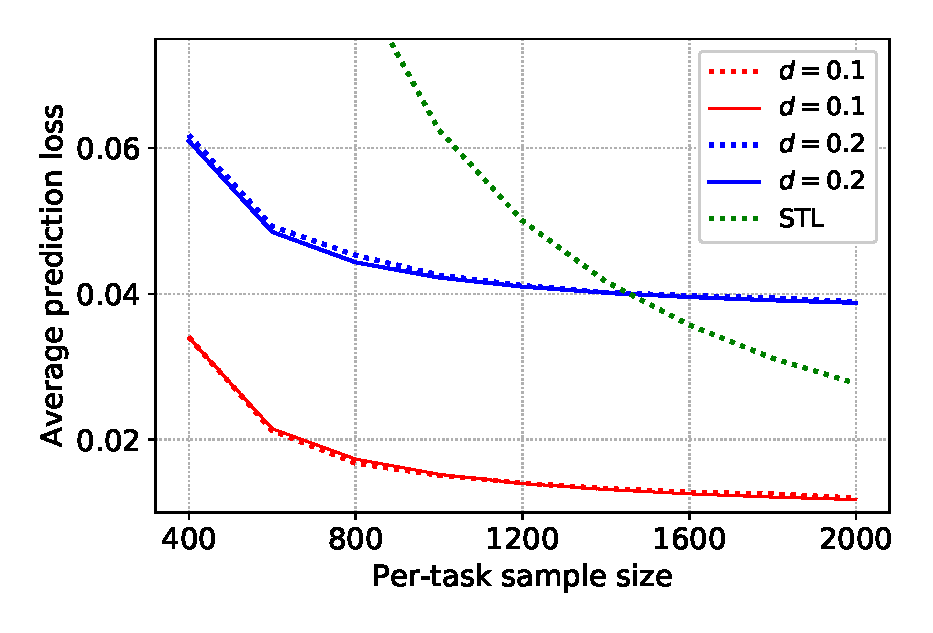
\includegraphics[width=0.95\textwidth]{figures/same_covariates.eps}
		\caption{Example \ref{ex_same_cov}}
		\label{fig_same_cov}
	\end{subfigure}\hfill
	\begin{subfigure}[b]{0.33\textwidth}
		\centering
		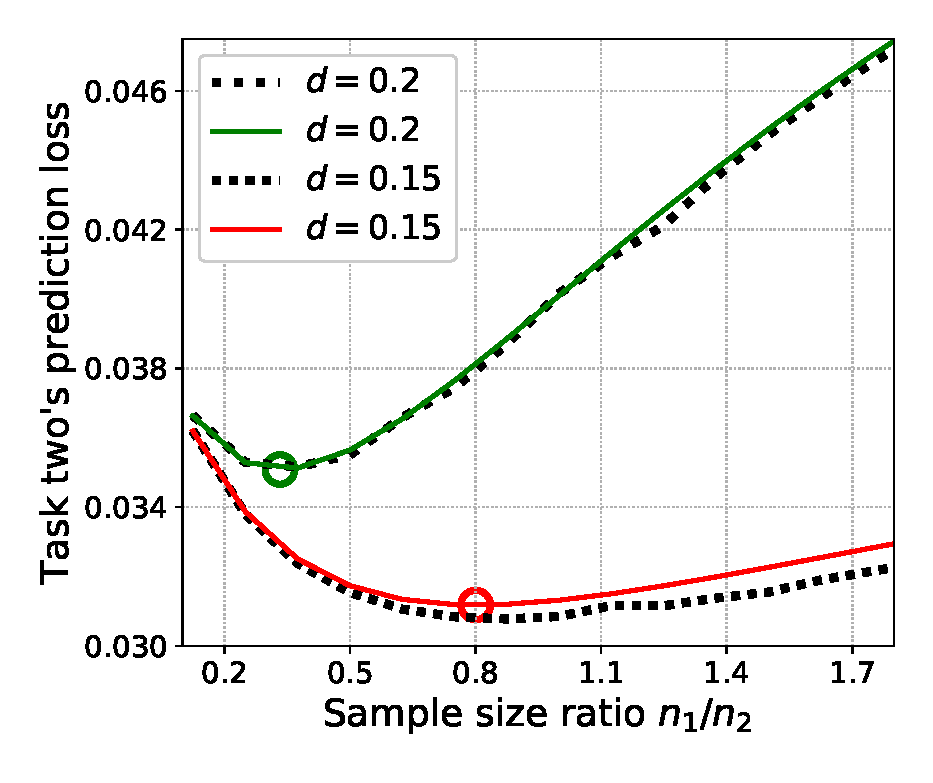
\includegraphics[width=0.95\textwidth]{figures/sample_ratio_several_d.eps}
		\caption{Example \ref{ex_sample_ratio}}
		\label{fig_size}
	\end{subfigure}\hfill
	\begin{subfigure}[b]{0.33\textwidth}
		\centering
		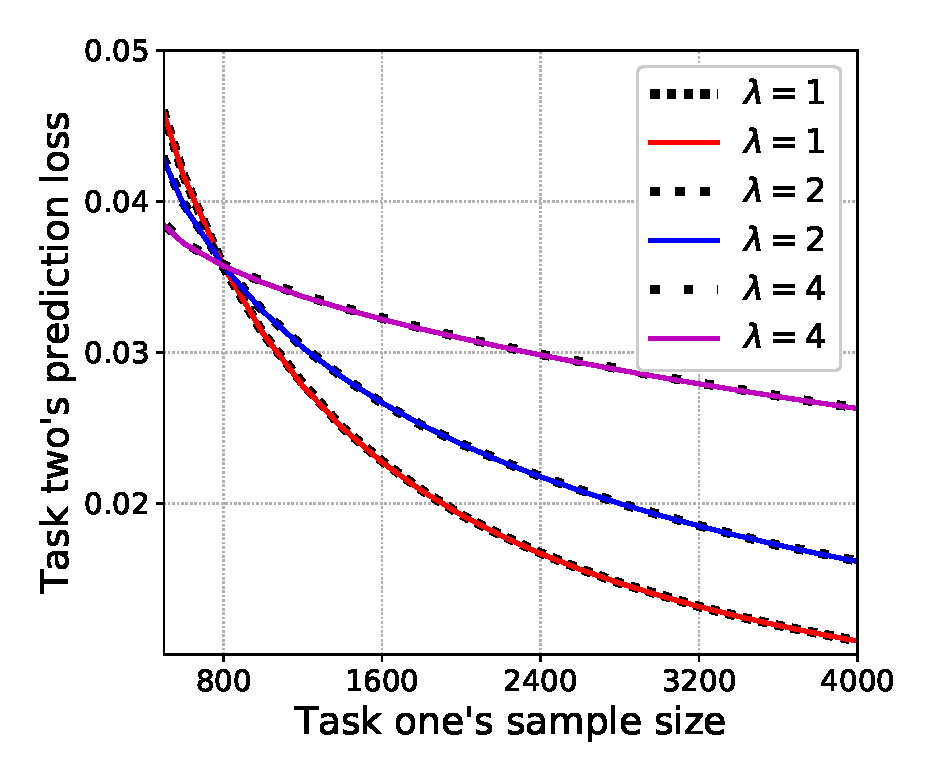
\includegraphics[width=0.95\textwidth]{figures/covariate_shift.eps}
		\caption{Example \ref{ex_covshift}}
		\label{fig_covariate}
	\end{subfigure}
	\caption{%Three takeaways of our theory in Section \ref{sec_insight}.
	Validating Example \ref{ex_same_cov} in Section \ref{sec_same} for $10$ tasks:
	In Figure \ref{fig_same_cov}, our estimated loss (solid line) matches the empirical loss (dotted line) accurately for various task-specific variance $d^2$ and sample size $n$ settings. The feature dimension $p$ is $200$, and noise variance $\sigma^2$ is $1/4$.
	Validating Example \ref{ex_sample_ratio} and Example \ref{ex_covshift} in Section \ref{sec_diff} for two tasks:
	in both experiments, our estimated losses (solid line) match the empirical losses (dotted line) accurately.
	In Figure \ref{fig_size}, we discover several interesting phenomena by fixing task two's sample size and increasing task one's sample size.
	Depending on how large $d^2$ is, task two's prediction loss decreases initially before increasing again, or decreases monotonically.
	In Figure \ref{fig_covariate}, we show how different levels of covariate shift affect hard parameter sharing when there is no bias.
	Having covariate shift increases task two's prediction loss when task two's sample size is larger than task one. Otherwise, having covariate shift (surprisingly) decreases task two's prediction loss.}
	\label{fig_model_shift_phasetrans}
\end{figure*}



%Recall that  $U\Lambda V^\top$ is the singular value decomposition of $M$, %$\Lambda$ consists of the singular values of $M$, $V$ is an orthonormal matrix,
%It is not hard to verify that $(n_1 + n_2)\hat{\Sigma}^{-1}= (\Sigma^{(2)})^{-1/2} V W^{-1}V^\top (\Sigma^{(2)})^{-1/2}$ and .
Let $\mu=p^{-1}\sum_{i} \delta_{\sigma_i}$ denote the empirical spectral distribution of $W$, where $\sigma_i$'s are the eigenvalues of $W$ and $\delta_{\sigma_i}$ is the point mass measure at $\sigma_i$. Then it is easy to see that the Stieltjes transform of $\mu$ is equal to
 \[ m_{\mu}(z) \define \frac{1}{p}\sum_{i=1}^p \frac{1}{\sigma_i - z}= p^{-1}\tr\left[(W-z\id)^{-1}\right]. \]
Above, the matrix $(W - z\id)^{-1}$ is known as $W$'s resolvent or Green's function.
%When $p$ goes to infinity, it is well-known that $m_{\mu}(z)$ converges to a fixed distribution governed by a set of self-consistent equations.
%These self-consistent equations give the asymptotic limit of the trace of $\hat{\Sigma}^{-1}$.
%The above approach applies when $\Sigma^{(2)}$ is isotropic in Theorem \ref{thm_main_RMT}.
%Since our goal is to show the limit of $\tr\left[ (Y - z\id)^{-1}V^{\top}{\Sigma^{(2)}}^{-1}V \right]$ as shown in equation \eqref{eigen2extra}, we study the  $(Y-z\id)^{-1}$.
%Compared to the Stieltjes transform, the resolvent also applies to random matrices.
We will prove the convergence of $W$'s resolvent using the so-called ``local laws'' with a sharp convergence rate \cite{isotropic,erdos2017dynamical,Anisotropic}.
%Recent developments in the random matrix literature have shown the convergence of the resolvent matrix using the so-called ``local laws'' or ``deterministic equivalents'' (cf. \cite{Hachem2007deterministic,DS18}).

%For our purpose, we use a convenient linearization trick in linear algebra, that is, the SVD of a rectangular matrix $A$ is equivalent to the study of the eigendecomposition of the symmetric block matrix
%$$H(A):=\begin{pmatrix}0 & A \\ A^\top & 0\end{pmatrix},$$
%which is linear in $A$. This trick has been used in many random matrix literatures, such as \cite{Anisotropic, AEK_Gram, XYY_circular,DY20201}.


